\textbf{\uline{Exemplo 01:}}
	\begin{center}
		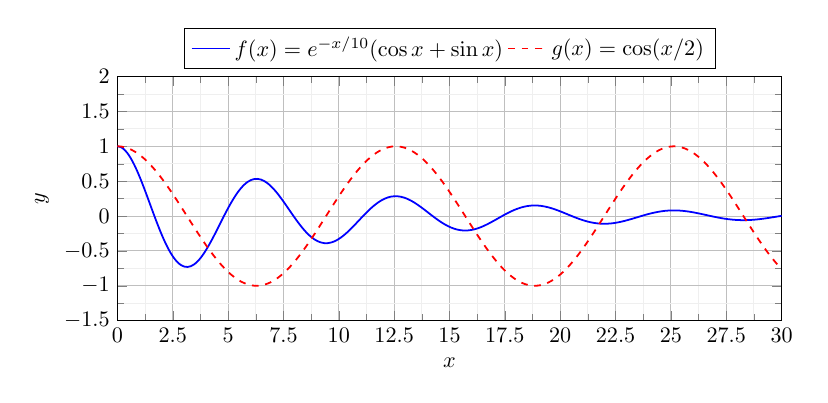
\begin{tikzpicture}[scale=0.8]
			\begin{axis}[
				xmin = 0, xmax = 30,
				ymin = -1.5, ymax = 2.0,
				%axis x line*=middle,
				xtick distance = 2.5,
				ytick distance = 0.5,
				grid = both,
				xlabel=$x$,
				ylabel=$y$,
				minor tick num = 1,
				major grid style = {lightgray},
				minor grid style = {lightgray!25},
				%legend style={at={(1.03,1)},anchor=north west,legend columns = 1},
				legend style={at={(0.5,1.03)},anchor=south,legend columns = 2},
				width = \textwidth,
				height = 0.45\textwidth]
				\addplot[
				domain = 0:30,
				samples = 200,
				smooth,
				thick,
				blue,
				] {exp(-x/10)*( cos(deg(x)) + sin(deg(x))/10 )};
				\addplot[
				domain = 0:30,
				samples = 200,
				smooth,
				thick,
				red,
				dashed,
				] {cos(0.5*deg(x))};
				\legend{$f(x)=e^{-x/10}(\cos x + \sin x)$,$g(x)=\cos(x/2)$}
			\end{axis}
		\end{tikzpicture}
	\end{center}1